
The task of vision subsystem is to handle the image data acquired from Raspbery Pi camera. This handling includes two basic subtasks: sign detection and sign recognition (classification).

Three basic signs detected and recognized by the system are shown on figure \ref{fig:raw-signs}. They are printed on a flat paper surface.

\begin{figure}[th!]
	\centering
	\begin{subfigure}[b]{0.2\textwidth}
		\centering
		
\includegraphics[scale=0.25]{sign-circle.png}
		\subcaption{Circle (goal)}
	\end{subfigure}
	\begin{subfigure}[b]{0.4\textwidth}
		\centering
		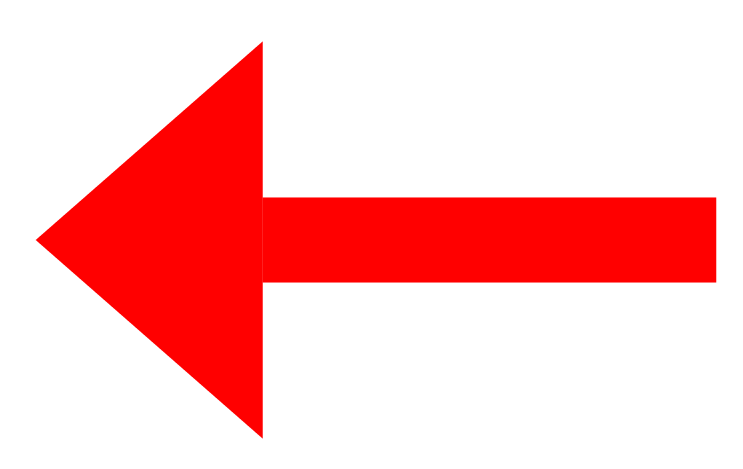
\includegraphics[scale=0.25]{sign-arrow.png}
		\subcaption{Arrow (direction change)}
	\end{subfigure}
	\begin{subfigure}[b]{0.2\textwidth}
		\centering
		
\includegraphics[scale=0.25]{sign-cross.png}
		\subcaption{Cross (stop)}
	\end{subfigure}
	\caption{Shape of signs used by the system}
	\label{fig:raw-signs}
\end{figure}

Basic workflow of the vision processing module is split into functional blocks, shown on the figure \ref{fig:vision-module-blocks}.

\begin{figure}[th!]
	\centering
		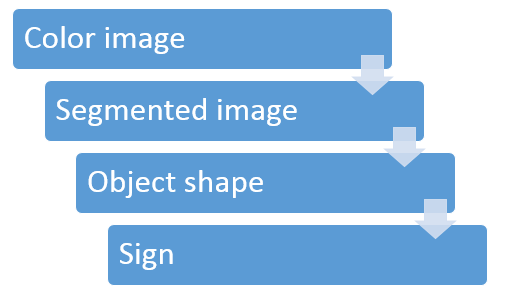
\includegraphics[scale=0.5]{image-module.png}
	\caption{Workflow of vision module}
	\label{fig:vision-module-blocks}
\end{figure}

Different methods and challenges encountered in vision module are described and discussed separately in the following chapters of the report.

\paragraph{Thresholding}

The first and the most intuitive approach to sign detection procedure was simple color thresholding, since signs which had to be detected are purely red.

The initial choice for color thresholding was HSV color space. Ranges of H (hue), S (saturation) and V (value) channels are [0,180], [0, 255] and [0, 255], respectively. In order to segment only red color, values of H (hue) channel greater than 170 and lower than 10 were used, since this range represents the band of red color. Additionally, too dark (V $ < $ 40), to bright (V $ > $ 220) and non-saturated pixels (S $ < $ 40) were rejected to improve the quality of segmentation. Results are shown on the figure ~\ref{fig:color-spaces}.

\begin{figure}[th!]
	\centering
	\begin{subfigure}[b]{0.3\textwidth}
		\centering
	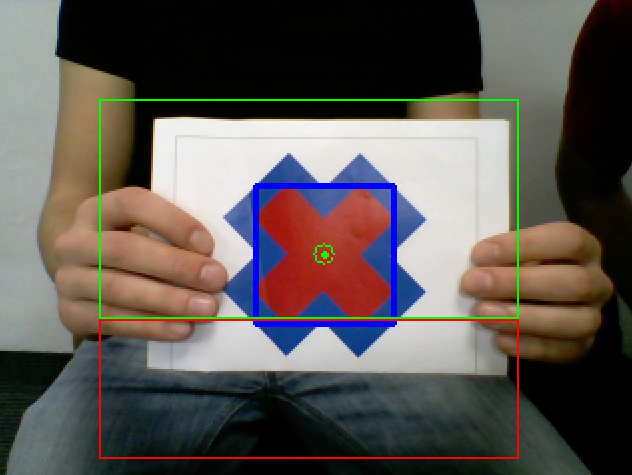
\includegraphics[scale=0.33]{thresholding-raw.png}
	\subcaption{Raw camera input}
	\end{subfigure}
	\begin{subfigure}[b]{0.3\textwidth}
		\centering
		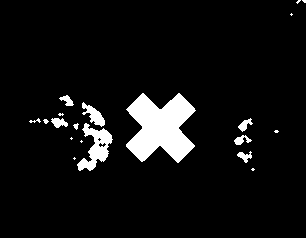
\includegraphics[scale=0.7]{thresholding-hsv.png}
		\subcaption{HSV color space}
	\end{subfigure}
	\begin{subfigure}[b]{0.3\textwidth}
		\centering
		\includegraphics[scale=0.7]{thresholding-YCrCb.png}
		\subcaption{YCrCb color space}
	\end{subfigure}
	\caption{Comparison of color spaces used for thresholding}
	\label{fig:color-spaces}
\end{figure}

After some testing, YCrCb color space proved to give better results for segmentation, as shown on figure above. As a result, YCrCb color space was used in final implementation.

Usage of IR camera did not affect the recognition quality of the thresholding procedure in regular, normal lighting conditions. On the other hand, it drastically increased the accuracy in low lighting conditions, which is described in Hardware section of the report.

The biggest connected component (blob) int he thresholded image is considered to be a sign. Bounding box of the biggest blob determined the area of the thresholded image to be passed in as an input to the sign classification module. 

\paragraph{Classification of the signs using statistical moments}

Taking into consideration the relatively low computational power of the hardware platform used to develop the system, priority for the chosen sign classification algorithm was low complexity.

After some thorough analysis of the available option, statistical moments proven to be the best option.

For an arbitrary binary (i.e. thresholded) input image system can compute statistical moments of desired order. The moment of importance in case of sign classification was center of mass or first order moment. It can be thought of average coordinate of all white pixels for both axes.

\begin{figure}[th!]
	\centering
	\begin{subfigure}[b]{0.25\textwidth}
		\centering
		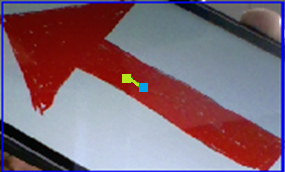
\includegraphics[scale=0.55]{moments-arrow-raw.png}
		\subcaption{Raw camera input}
	\end{subfigure}
	\begin{subfigure}[b]{0.25\textwidth}
		\centering
		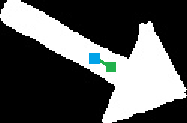
\includegraphics[scale=0.8]{moments-arrow-segm.png}
		\subcaption{Arrow}
	\end{subfigure}
	\begin{subfigure}[b]{0.2\textwidth}
		\centering
		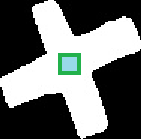
\includegraphics[scale=0.8]{moments-cross-segm.png}
		\subcaption{Cross}
	\end{subfigure}
	\begin{subfigure}[b]{0.2\textwidth}
		\centering
		
\includegraphics[scale=0.9]{moments-circle-segm.png}
		\subcaption{Circle}
	\end{subfigure}
	\caption{Visual cues for sign classification using statistical moments}
	\label{fig:statistical-moments}
\end{figure}

Figure \ref{fig:statistical-moments} demonstrates intuition behind visual cues used for discrimination of three different types of signs. By computing the distance of center of the mass (green rectangle) and center of the cropped image segment where the sign was detected (blue rectangle) we can perform initial discrimination between \textbf{arrow} and \textbf{rest two signs}. Distance is going to be close to zero in case of cross and circle since object are symmetrical around two mutually normal axes. Arrow is not symmetrical around one axis, so it's center of the mass will be slightly shifter towards the tip of the arrow and this is the property used to distinguish an arrow from the circle and cross.
Table \ref{tab:moments} shows average distance of center of the mass from image center proportional to cropped image size. Clear observation is that thresholding this distance to 10 $\%$ can give is pretty good estimate of probability that sign belongs to arrow class.

If this distance is close to zero, additional step is needed to determine is the observed sign cross or circle. Approach used in this step was investigation of zero-order moment, which gives the number of white pixels in the image. By taking the ratio of zero order moment and total number of pixels of sign area, we can distinguish between cross and circle. Intuition behind this metric lies in the fact that circle has bigger surface than cross of the same bounding box size, so the percentage of space it occupies in the cropped image area where the sign is going to be larger than if it was cross. Table \ref{tab:moments} gives suitable value of threshold of 70 $\%$.

\begin{table}[th!]
\centering
\begin{tabular}{l*{2}{c}r}
	Sign class			& Distance of first moment & Ratio of second order moment  \\
	\hline
	Arrow 				& 18.41 & 56.44  \\
	Cross            	& 1.39 & 54.20  \\
	Circle           	& 0.97 & 89.63  \\
\end{tabular}
\caption{Numerical values of statistical moments given in $\%$ wrt. image size}
\label{tab:moments}
\end{table}

Described method proved to be sufficiently accurate for practical purposes, while still remaining \textbf{computationally tractable} on available hardware. More robust classification methods will be discussed in section \ref{sec:future-improvements} and are subject to future investigation.

\paragraph{Neural network classifier}

Justification of usage neural networks.

Very brief theoretical background.

Description of the way how we train it on images (raw pixel values, segmentation pixels, hu-moments as inputs, etc)

Description of tested recognition method (sliding window, random, ...)

Performance comparison with previous method.

\paragraph{Computing arrow orientation}

After sign has been classified as arrow, additional step needs to be performed in order to extract the arrow angle relative to the orientation of the robot at the moment of observation.

Initial idea was to use already computed information about the statistical moments to get the orientation of the arrow. Center of the mass and center of the cropped image segment containing the sign form a vector pointing towards tip of the arrow. We can exploit this information to determine the angle of the vector, as shown on figure \ref{fig:arrow-angle-computation}. Although not so robust, this was intuitive and the fastest method to prototype since all moments are already computed for sign classification step, which meant that this method would reduce computational overhead.

\begin{figure}[th!]
	\centering
	\begin{subfigure}[b]{0.45\textwidth}
		\centering
		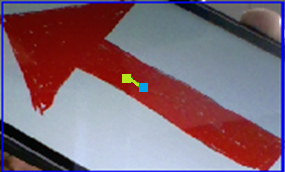
\includegraphics[scale=0.7]{moments-arrow-raw.png}
		\subcaption{Raw camera input}
	\end{subfigure}
	\begin{subfigure}[b]{0.45\textwidth}
		\centering
		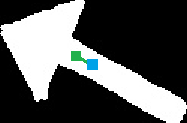
\includegraphics[scale=1]{moments-arrow-segm-angle.png}
		\subcaption{Arrow}
	\end{subfigure}
		\begin{subfigure}[b]{0.45\textwidth}
			\centering
			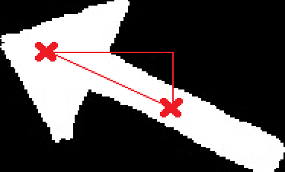
\includegraphics[scale=0.7]{moments-arrow-segm-angle-math.png}
			\subcaption{Angle from moments}
		\end{subfigure}
		\begin{subfigure}[b]{0.45\textwidth}
			\centering
			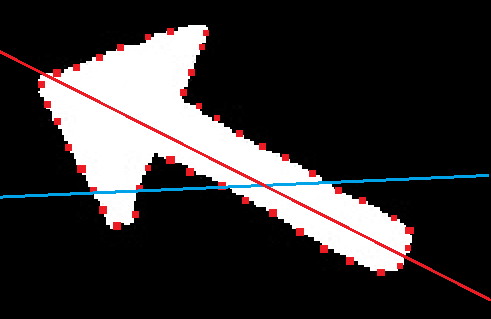
\includegraphics[scale=0.55]{moments-arrow-segm-angle-fitting.png}
			\subcaption{Line fitting}
			\label{fig:line-fitting}
		\end{subfigure}
	\caption{Computation of the arrow orientation}
	\label{fig:arrow-angle-computation}
\end{figure}

After implementation and extensive testing of mentioned method, some scenarios where it fails were met. One of them is shown in the figure , where wrong value of the angle is computed or it wasn't reliable enough (it was oscillating a lot). Oscillation problem could have been solved by filtering, but instead a different approach was chosen.

Instead of focusing on statistical properties of the contour of the arrow better approach is to utilize the whole information about it's contour. Contour of the arrow shape is extracted from segmented binary image of the arrow. Array of points representing the contour is then fitted to the line in \textbf{Linear Least Squares fashion (LLS)}, which is a well known function minimization framework for linear systems.

The basic idea is posing the problem of finding unknown arrow angle $\theta$ as function minimization problem, where input is defined as set $C$ of $N$ contour points $C_i \in \mathbb{R}^2$. Cost function on a set of points $C$ and chosen angle $\theta$ is defined as sum of the squared distance of each contour point $C_i$ from the line with angle $\theta$, which is formally given by equation \ref{eq:LLS}. Minimizing this function over $\theta$ gives the optimal line angle that fits the given contour points.

\begin{equation}
f(C,\theta)=
\frac{1}{N}
\sum_{i=1}^{N}distance(C_i, line(\theta))^2
\label{eq:LLS}
\end{equation}

Figure \ref{fig:line-fitting} shows two arbitrary lines on top of the segmented image of the arrow. Blue line has higher value of the cost function than the red line because it doesn't fit the given data (contour points) the best possible way. Red line is the optimal angle for given shape, determined by least square solution of the equation \ref{eq:LLS}.

OpenCV has LLS implementation of described line fitting algorithm, which was used in the final version of the solution. Using this method improved the accuracy and stability of orientation of the arrow without significant impact on performance, since optimization problem can be solved using techniques linear algebra, which are computationally inexpensive.

\paragraph{Solving partial occlusion and re-detection}

Problem of partial occlusion arises when robot is moving forward and a sign is slowly getting into the area observed by robot. Some time is needed before the sign completely enters the view and attempt of classification partially visible sign would result in misclassification in most of te cases.

Also, there is a problem of detecting proximity of the robot to the observed sign, because desired behavior is to switch states only when the robot is close to sign it detects and not as soon it detects it.

In order to prevent attempts of classifications of partially visible signs and detecting proximity of the robot to the sign, whole view of the camera is split into two regions of interest: \textbf{perceptive area} and \textbf{proximity area}, shown on figure \ref{fig:camera-view-areas}. Using these view areas system is able to overcome the described problems in very easy and intuitive way.

\begin{figure}[th!]
	\centering
		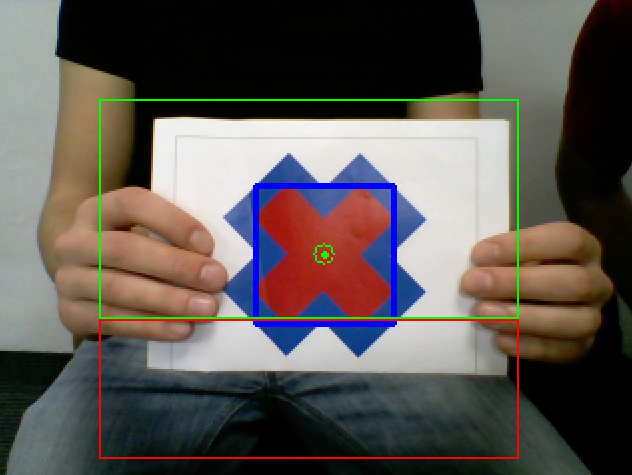
\includegraphics[scale=0.5]{thresholding-raw.png}
	\caption{Perceptive (green) and proximity (red) area}
	\label{fig:camera-view-areas}
\end{figure}

Detection of the sign (segmentation and blob detection) are performed at every iteration and position of the object is extracted as center of the detected blob. For predefined camera position and physical size of the signs, it can be assumed that \textbf{if object's center is inside the perception area it will be completely inside the camera view}. This allows reliable determination of exact classification moment, without risk of classifying partially visible objects.

Similar strategy is used for detecting the proximity of the sign: if it's center is in the proximity area it is assumed to be close to the robot. Since slightly delayed image processing and low FPS, it will take some time for robot to determine that it approached the sign. This will result in robot ending up exactly on the sign at the moment when it switches to execution of the command defined by the sign.
